\RequirePackage[l2tabu, orthodox]{nag}
\documentclass[12pt]{article}

\usepackage{amssymb,amsmath,verbatim,graphicx,microtype,upquote,units,booktabs,siunitx}

\title{Test II Study Guide}
\date{\today}
\author{Illya Starikov}

\begin{document}
\maketitle

\section{Notes}
\begin{itemize}
    \item If a dielectric fills one half a the space between plates, it's the same as two capacitors in parallel --- one with a dielectric, one not.
    \item Current is in the direction of flow of \textbf{positive charge}.
    \item Materials that are ohmic have a linear $I$ vs. $V$ graph.
    \begin{itemize}
        \item Anything else (like quadratic) are nonohmic.
    \end{itemize}

    \item For resistors \textbf{in series},
    \begin{itemize}
        \item $R_{eq} = \sum _i R_i$ (opposite of capacitors)
        \item Currents $I$ is the same (same as capacitors)
        \item $V$'s add (same as capacitors)
    \end{itemize}

    \item For resistors \textbf{in parallel},
    \begin{itemize}
        \item $\frac{1}{R_{eq}} = \sum _i \frac{1}{R_i}$ (opposite of capacitors)
        \item Currents $I$ is the same (same as capacitors)
        \item $V$'s add (same as capacitors)
    \end{itemize}

    \item Power = $\frac{\text{Energy Transformed}}{\text{Time}}$
    \item Kirchhoff’s Junction Rule: at any junction point, the sum of all currents entering the junction must equal the sum of all currents leaving the junction.
    \item Kirchhoff’s Loop Rule: the sum of the changes of potential around any closed path of a circuit must be zero.
\end{itemize}

\frame{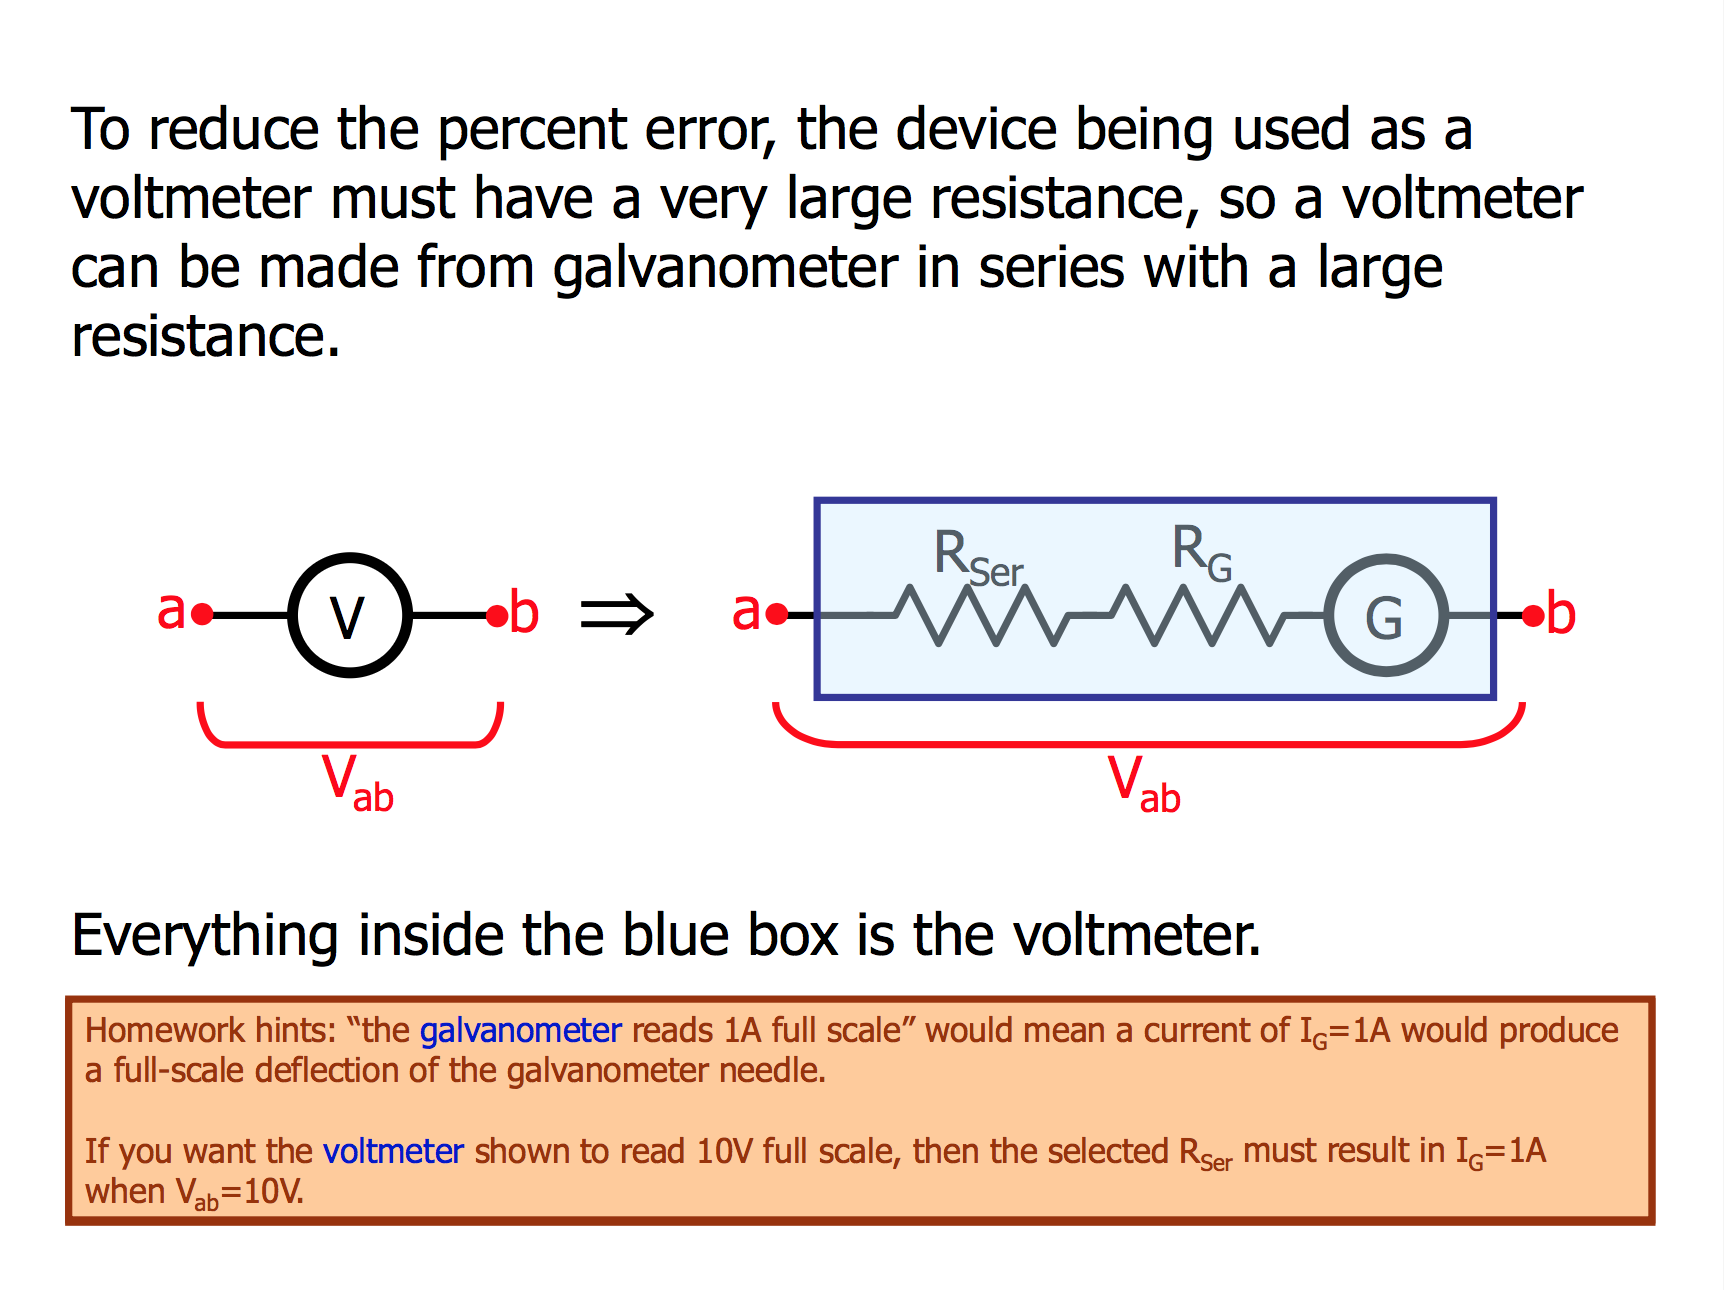
\includegraphics[width=\columnwidth]{assets/voltmeter}}
\frame{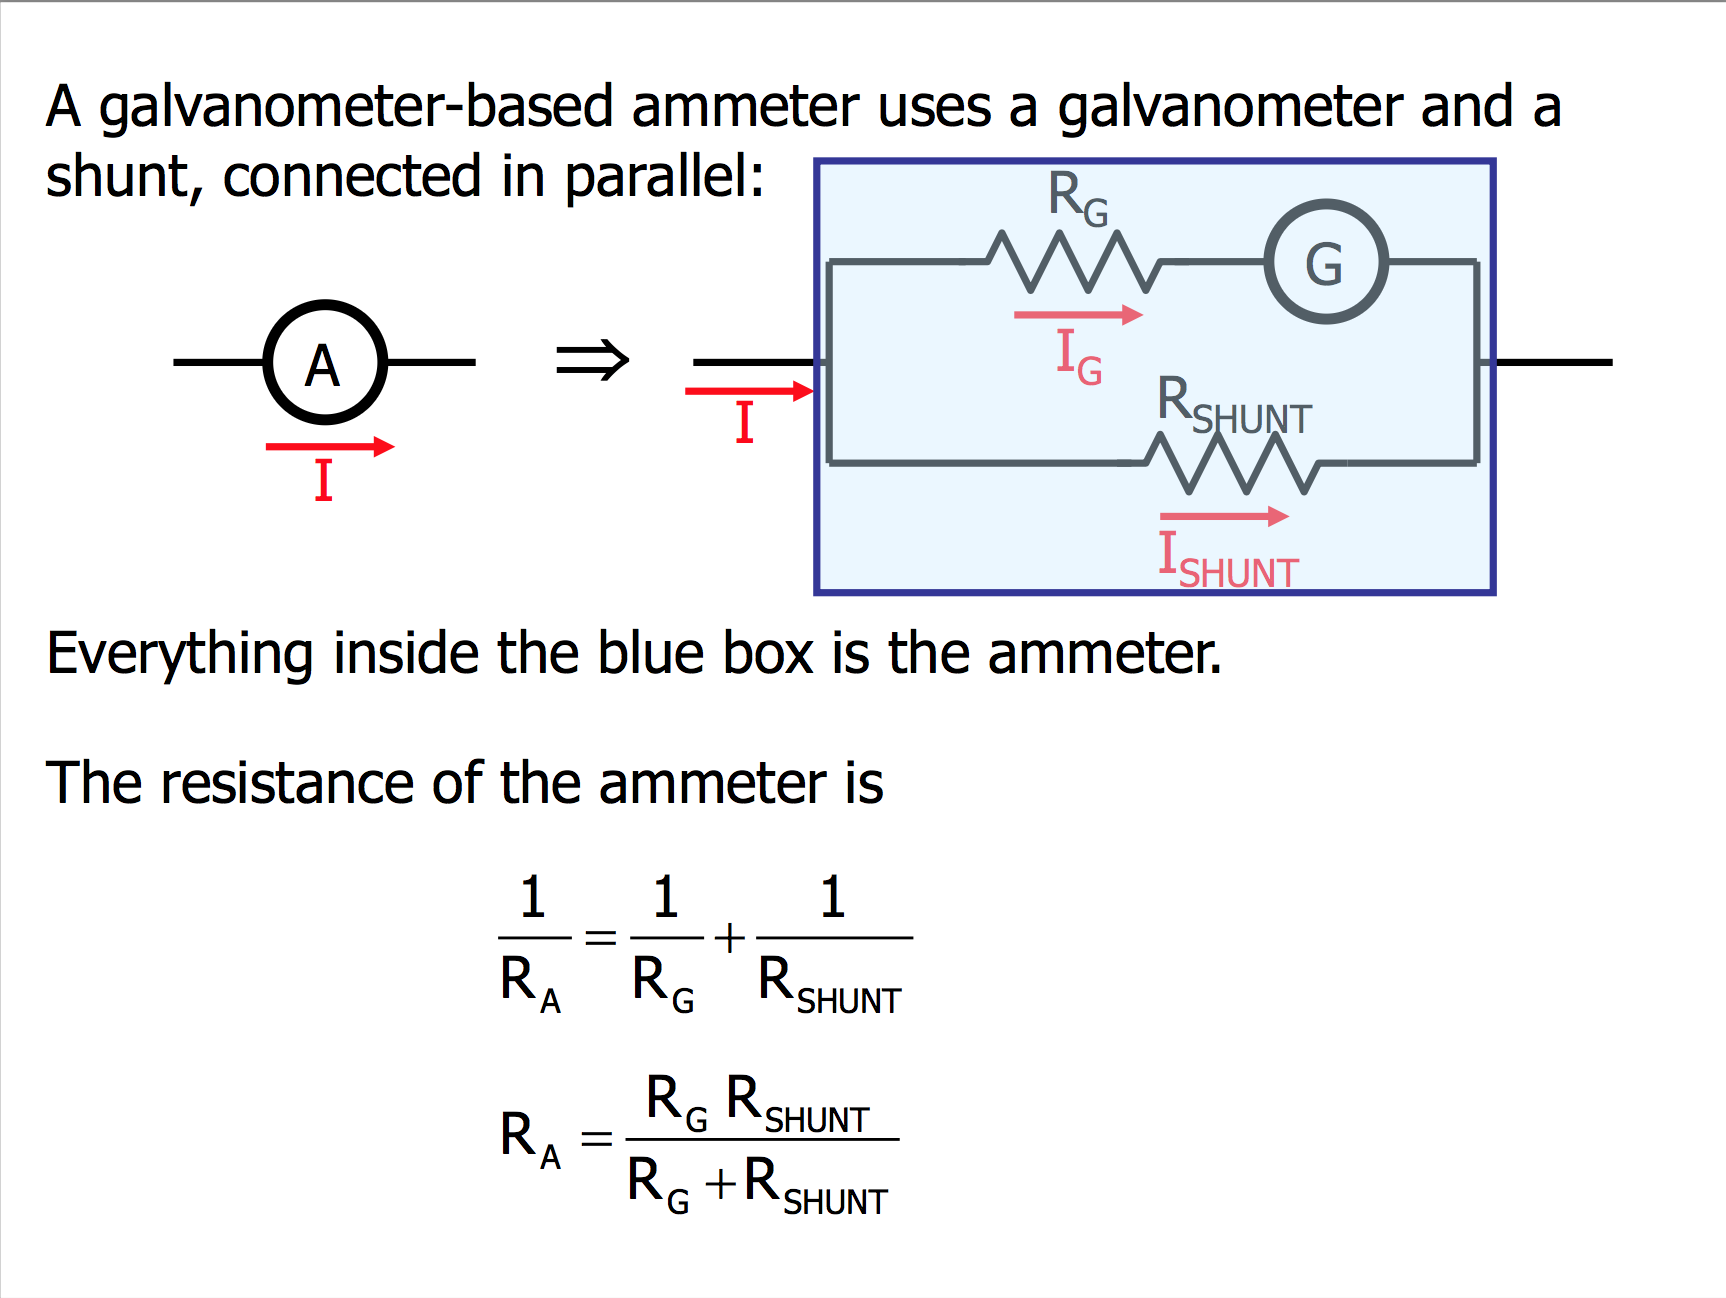
\includegraphics[width=\columnwidth]{assets/ammeter}}

\begin{itemize}
    \item For charging a circuit, $I(t) = \frac{\varepsilon}{R} e^{-\frac{t}{RC}}$
    \item For discharging a circuit, $I(t) = I_0 e^{-\frac{t}{RC}}$
    \begin{itemize}
        \item $I_0$ for charging is equal to $I_0$ for discharging only if the discharging capacitor was fully charged.
    \end{itemize}

    \item In a series RC circuit, the same current $I$ flows through both the capacitor and the resistor. Sometimes this fact comes in handy.
    \item Ohm's law \textbf{only} applies to resistors, not capacitors.

    \item Magnetic field lines point away from north, towards south.
    \begin{itemize}
        \item Same notation as electric fields!
    \end{itemize}

    \item In a uniform magnetic field, force is always radially outward. Therefore, $a = \nicefrac{v^2}{r}$.
    \begin{itemize}
        \item Period $T = \frac{2 \pi r}{v}$. (However, easier to remember $\text{distance} = \text{velocity} \cdot \text{time} \implies T = \frac{\text{distance}}{\text{velocity}}$)
        \item frequency = $\frac{1}{T}$
    \end{itemize}
\end{itemize}

\section{Units}
\begin{itemize}
    \item Resistance: $1 \Omega = \frac{1 V}{1 A}$
    \item Resistivity: $\rho = \Omega \cdot m$
    \item Magnetic field: $1 T = \frac{\SI{1}{kg}}{\text{C} \cdot \text{s}}$
    \item Older unit: $\SI{1}{G} = 10^{-4}\text{T} $
\end{itemize}

\section{Unit Prefixes}
\begin{center}
    \begin{tabular}{|l|l|}
        \hline
        $10^{-15}$ & femto	($f$)    \\ \hline
        $10^{-12}$ & pico	($p$)    \\ \hline
        $10^{-9}$  & nano	($n$)    \\ \hline
        $10^{-6}$  & micro	($\mu$)  \\ \hline
        $10^{-3}$  & milli	($m$)    \\ \hline
        $10^{-2}$  & centi	($c$)    \\ \hline
        $10^{-1}$  & deci	($d$)    \\ \hline
    \end{tabular}
\end{center}

\end{document}
